%%__________________________________________________________________||
\section{Results and interpretation}
\label{sec:interpretation}

A likelihood model of the observations in all data samples is
used to obtain a consistent prediction of the SM backgrounds and to
test for the presence of a variety of signal models.

In each bin of \scalht, the observation is modelled as a
Poisson-distributed variable around the sum of the SM expectation and a
potential signal contribution (assumed to be zero in the following
discussion). The SM expectation is related to the expected yields in
the \mj, \mmj, and \gj control samples via the transfer factors
derived from simulation. Likelihood functions describe the yields in the \scalht bins
of the \mj, \mmj, and \gj control samples in the same category of
\njet and \nb as the signal region. The systematic uncertainties
associated with the transfer factors are accommodated in the
likelihood function by a nuisance parameter per transfer factor. The
measurements of these parameters are assumed to follow a log-normal
distribution. The CL$_{\mathrm{s}}$ technique~\cite{read, Cowan:2010js} was used to set limits using asymptotic formulae.

The expected number of events from SM processes is determined from a
simultaneous fit to the signal region and up to three control
samples. The likelihood function is maximised over all fit parameters
under the SM-only hypothesis.
Tables~\ref{tab:yieldsewkdatapost_sig_comb_sym} and \ref{tab:yieldsewkdatapost_sig_comb_asym} and
\ref{tab:yieldsewkdatapost_sig_comb_mono} summarise
the observed yields and fit results with associated errors in bins of \scalht for events in the signal region
categorised according to \njet and \nb. 
No significant tension is observed between the predictions and data in the
signal region which is well described by the SM-only hypothesis.

\begin{table}[h!]
\tiny
\centering
\caption{Predictions and Data in the signal region for 1.26\ifb for symmetric categories. The letter ``a'' in jet \eg ``2a''  indicates the asymmetric jet bins. All entries are non-zero but are truncated to one decimal place.\label{tab:yieldsewkdatapost_sig_comb_sym}}
\begin{tabular}
{cccccccccc}
	\hline\hline
&	&	& \multicolumn{8}{c}{\scalht (\gev)}\\ 
	&	 (\njet, \nb) & 200-250 & 250-300 & 300-350 & 350-400 & 400-500 & 500-600 & 600-800 & 800-$\infty$ \\ [0.8ex] 
\hline
	SM & (2, 0) & $559.6^{+ 25.3 }_{- 25.3 }$ & $599.0^{+ 27.4 }_{- 27.4 }$ & $398.0^{+ 19.7 }_{- 19.7 }$ & $246.9^{+ 18.0 }_{- 18.0 }$ & $196.5^{+ 12.9 }_{- 12.9 }$ & $53.6^{+ 7.4 }_{- 7.4 }$ & $36.8^{+ 5.6 }_{- 5.6 }$ & $30.7^{+ 4.8 }_{- 4.8 }$ \\[0.5ex] 
	Data & (2, 0) & 552 & 592 & 395 & 247 & 189 & 55 & 39 & 33 \\[0.5ex] 
	SM & (2, 1) & $73.7^{+ 7.0 }_{- 7.0 }$ & $57.2^{+ 6.2 }_{- 6.2 }$ & $32.7^{+ 4.6 }_{- 4.6 }$ & $22.0^{+ 4.0 }_{- 4.0 }$ & $16.5^{+ 2.4 }_{- 2.4 }$ & $4.1^{+ 1.3 }_{- 1.3 }$ & $2.9^{+ 1.0 }_{- 1.0 }$ & $3.2^{+ 0.9 }_{- 0.9 }$ \\[0.5ex] 
	Data & (2, 1) & 81 & 63 & 35 & 22 & 23 & 3 & 1 & 2 \\[0.5ex] 
	SM & (2, 2) & $1.6^{+ 1.2 }_{- 1.2 }$ & $1.8^{+ 1.3 }_{- 1.3 }$ & $1.2^{+ 0.8 }_{- 0.8 }$ & -- & $1.0^{+ 0.4 }_{- 0.4 }$ & $0.3^{+ 0.3 }_{- 0.3 }$ & $0.2^{+ 0.2 }_{- 0.2 }$ & $0.1^{+ 0.2 }_{- 0.2 }$ \\[0.5ex] 
	Data & (2, 2) & 2 & 3 & 2 & -- & 2 & 0 & 0 & 0 \\[0.5ex] 
	SM & (3, 0) & $1.4^{+ 1.9 }_{- 1.9 }$ & $111.2^{+ 10.7 }_{- 10.7 }$ & $282.0^{+ 16.7 }_{- 16.7 }$ & $280.0^{+ 16.0 }_{- 16.0 }$ & $348.4^{+ 20.3 }_{- 20.3 }$ & $121.4^{+ 9.7 }_{- 9.7 }$ & $53.1^{+ 6.3 }_{- 6.3 }$ & $46.1^{+ 4.6 }_{- 4.6 }$ \\[0.5ex] 
	Data & (3, 0) & 1 & 111 & 283 & 282 & 353 & 120 & 51 & 51 \\[0.5ex] 
	SM & (3, 1) & $1.4^{+ 1.4 }_{- 1.4 }$ & $24.3^{+ 4.0 }_{- 4.0 }$ & $45.0^{+ 5.0 }_{- 5.0 }$ & $57.1^{+ 6.0 }_{- 6.0 }$ & $42.5^{+ 6.0 }_{- 6.0 }$ & $15.3^{+ 2.5 }_{- 2.5 }$ & $9.0^{+ 2.1 }_{- 2.1 }$ & $5.5^{+ 1.1 }_{- 1.1 }$ \\[0.5ex] 
	Data & (3, 1) & 2 & 25 & 49 & 60 & 35 & 16 & 10 & 5 \\[0.5ex] 
	SM & (3, 2) & -- & $4.4^{+ 1.2 }_{- 1.2 }$ & $9.0^{+ 1.9 }_{- 1.9 }$ & $8.2^{+ 1.7 }_{- 1.7 }$ & $6.8^{+ 1.4 }_{- 1.4 }$ & $2.1^{+ 0.6 }_{- 0.6 }$ & $0.9^{+ 0.3 }_{- 0.3 }$ & $0.2^{+ 0.2 }_{- 0.2 }$ \\[0.5ex] 
	Data & (3, 2) & -- & 4 & 4 & 4 & 9 & 3 & 2 & 0 \\[0.5ex] 
	SM & (3, $\ge3$) & -- & -- & -- & $0.7^{+ 0.8 }_{- 0.8 }$ & $0.2^{+ 0.2 }_{- 0.2 }$ & $0.1^{+ 0.1 }_{- 0.1 }$ & -- & -- \\[0.5ex] 
	Data & (3, $\ge3$) & -- & -- & -- & 0 & 1 & 0 & -- & -- \\[0.5ex] 
	SM & (4, 0) & -- & -- & $30.5^{+ 5.7 }_{- 5.7 }$ & $95.1^{+ 9.7 }_{- 9.7 }$ & $167.5^{+ 11.0 }_{- 11.0 }$ & $91.4^{+ 9.8 }_{- 9.8 }$ & $60.7^{+ 7.8 }_{- 7.8 }$ & $31.4^{+ 3.7 }_{- 3.7 }$ \\[0.5ex] 
	Data & (4, 0) & -- & -- & 31 & 93 & 158 & 92 & 60 & 33 \\[0.5ex] 
	SM & (4, 1) & -- & -- & $9.7^{+ 3.1 }_{- 3.1 }$ & $43.5^{+ 6.0 }_{- 6.0 }$ & $58.2^{+ 5.9 }_{- 5.9 }$ & $16.8^{+ 3.4 }_{- 3.4 }$ & $10.9^{+ 2.2 }_{- 2.2 }$ & $7.3^{+ 1.0 }_{- 1.0 }$ \\[0.5ex] 
	Data & (4, 1) & -- & -- & 7 & 44 & 64 & 14 & 10 & 5 \\[0.5ex] 
	SM & (4, 2) & -- & -- & $2.8^{+ 1.4 }_{- 1.4 }$ & $15.0^{+ 3.0 }_{- 3.0 }$ & $19.2^{+ 2.7 }_{- 2.7 }$ & $4.5^{+ 1.2 }_{- 1.2 }$ & $2.3^{+ 0.6 }_{- 0.6 }$ & $1.4^{+ 0.3 }_{- 0.3 }$ \\[0.5ex] 
	Data & (4, 2) & -- & -- & 5 & 15 & 24 & 7 & 4 & 0 \\[0.5ex] 
	SM & (4, $\ge3$) & -- & -- & -- & $1.4^{+ 0.9 }_{- 0.9 }$ & $1.1^{+ 0.7 }_{- 0.7 }$ & $0.4^{+ 0.3 }_{- 0.3 }$ & $0.1^{+ 0.1 }_{- 0.1 }$ & $0.0^{+ 0.0 }_{- 0.0 }$ \\[0.5ex] 
	Data & (4, $\ge3$) & -- & -- & -- & 3 & 0 & 0 & 0 & 0 \\[0.5ex] 
	SM & ($\ge5$, 0) & -- & -- & -- & $4.0^{+ 2.0 }_{- 2.0 }$ & $54.1^{+ 6.8 }_{- 6.8 }$ & $45.4^{+ 6.6 }_{- 6.6 }$ & $41.8^{+ 5.6 }_{- 5.6 }$ & $31.6^{+ 3.8 }_{- 3.8 }$ \\[0.5ex] 
	Data & ($\ge5$, 0) & -- & -- & -- & 5 & 55 & 47 & 41 & 36 \\[0.5ex] 
	SM & ($\ge5$, 1) & -- & -- & -- & $1.3^{+ 0.9 }_{- 0.9 }$ & $31.4^{+ 4.5 }_{- 4.5 }$ & $18.1^{+ 3.1 }_{- 3.1 }$ & $14.9^{+ 3.0 }_{- 3.0 }$ & $10.9^{+ 1.8 }_{- 1.8 }$ \\[0.5ex] 
	Data & ($\ge5$, 1) & -- & -- & -- & 1 & 34 & 17 & 16 & 13 \\[0.5ex] 
	SM & ($\ge5$, 2) & -- & -- & -- & $0.8^{+ 0.6 }_{- 0.6 }$ & $11.7^{+ 2.5 }_{- 2.5 }$ & $9.0^{+ 1.9 }_{- 1.9 }$ & $4.6^{+ 1.2 }_{- 1.2 }$ & $2.7^{+ 0.6 }_{- 0.6 }$ \\[0.5ex] 
	Data & ($\ge5$, 2) & -- & -- & -- & 0 & 9 & 9 & 5 & 4 \\[0.5ex] 
	SM & ($\ge5$, $\ge3$) & -- & -- & -- & -- & $0.9^{+ 0.5 }_{- 0.5 }$ & $0.4^{+ 0.3 }_{- 0.3 }$ & $0.7^{+ 0.4 }_{- 0.4 }$ & $0.3^{+ 0.1 }_{- 0.1 }$ \\[0.5ex] 
	Data & ($\ge5$, $\ge3$) & -- & -- & -- & -- & 0 & 0 & 0 & 3 \\[0.5ex] 
	\hline
	\hline
\end{tabular}
\end{table}

\begin{table}[h!]
\tiny
\centering
\caption{Predictions and Data in the signal region for 1.26\ifb for asymmetric categories. The letter ``a'' in jet \eg ``2a''  indicates the asymmetric jet bins. All entries are non-zero but are truncated to one decimal place.\label{tab:yieldsewkdatapost_sig_comb_asym}}
\begin{tabular}
{cccccccccc}
	\hline\hline
&	&	& \multicolumn{8}{c}{\scalht (\gev)}\\ 
	&	 (\njet, \nb) & 200-250 & 250-300 & 300-350 & 350-400 & 400-500 & 500-600 & 600-800 & 800-$\infty$ \\ [0.8ex] 
\hline
	SM & (2a, 0) & $2894.8^{+ 53.6 }_{- 53.6 }$ & $854.8^{+ 28.8 }_{- 28.8 }$ & $293.3^{+ 16.3 }_{- 16.3 }$ & $141.9^{+ 11.4 }_{- 11.4 }$ & $83.3^{+ 9.1 }_{- 9.1 }$ & $11.3^{+ 3.3 }_{- 3.3 }$ & $7.7^{+ 3.1 }_{- 3.1 }$ & -- \\[0.5ex] 
	Data & (2a, 0) & 2887 & 857 & 290 & 143 & 83 & 11 & 8 & -- \\[0.5ex] 
	SM & (2a, 1) & $246.7^{+ 12.6 }_{- 12.6 }$ & $81.7^{+ 6.3 }_{- 6.3 }$ & $25.2^{+ 3.3 }_{- 3.3 }$ & $12.4^{+ 2.5 }_{- 2.5 }$ & $6.1^{+ 1.3 }_{- 1.3 }$ & $0.9^{+ 0.5 }_{- 0.5 }$ & $0.3^{+ 0.4 }_{- 0.4 }$ & -- \\[0.5ex] 
	Data & (2a, 1) & 254 & 77 & 29 & 12 & 7 & 1 & 0 & -- \\[0.5ex] 
	SM & (2a, 2) & $14.5^{+ 2.5 }_{- 2.5 }$ & $3.5^{+ 0.9 }_{- 0.9 }$ & $2.5^{+ 0.9 }_{- 0.9 }$ & $1.7^{+ 0.7 }_{- 0.7 }$ & $0.6^{+ 0.3 }_{- 0.3 }$ & $0.0^{+ 0.3 }_{- 0.3 }$ & $0.1^{+ 0.2 }_{- 0.2 }$ & -- \\[0.5ex] 
	Data & (2a, 2) & 15 & 6 & 2 & 1 & 0 & 0 & 0 & -- \\[0.5ex] 
	SM & (3a, 0) & $743.4^{+ 26.9 }_{- 26.9 }$ & $792.7^{+ 27.2 }_{- 27.2 }$ & $374.0^{+ 19.0 }_{- 19.0 }$ & $125.3^{+ 10.4 }_{- 10.4 }$ & $52.9^{+ 6.9 }_{- 6.9 }$ & $10.0^{+ 3.5 }_{- 3.5 }$ & $3.4^{+ 2.0 }_{- 2.0 }$ & -- \\[0.5ex] 
	Data & (3a, 0) & 739 & 798 & 372 & 118 & 55 & 11 & 3 & -- \\[0.5ex] 
	SM & (3a, 1) & $148.4^{+ 10.7 }_{- 10.7 }$ & $143.4^{+ 9.8 }_{- 9.8 }$ & $62.6^{+ 7.1 }_{- 7.1 }$ & $27.0^{+ 4.7 }_{- 4.7 }$ & $6.3^{+ 1.6 }_{- 1.6 }$ & $0.9^{+ 0.6 }_{- 0.6 }$ & $0.7^{+ 0.8 }_{- 0.8 }$ & -- \\[0.5ex] 
	Data & (3a, 1) & 152 & 135 & 66 & 35 & 5 & 0 & 1 & -- \\[0.5ex] 
	SM & (3a, 2) & $25.7^{+ 3.5 }_{- 3.5 }$ & $25.0^{+ 2.9 }_{- 2.9 }$ & $13.9^{+ 2.4 }_{- 2.4 }$ & $5.7^{+ 1.6 }_{- 1.6 }$ & $0.9^{+ 0.4 }_{- 0.4 }$ & $0.2^{+ 0.2 }_{- 0.2 }$ & $0.0^{+ 0.1 }_{- 0.1 }$ & -- \\[0.5ex] 
	Data & (3a, 2) & 25 & 28 & 12 & 5 & 0 & 0 & 0 & -- \\[0.5ex] 
	SM & (3a, $\ge3$) & $0.5^{+ 0.3 }_{- 0.3 }$ & $0.8^{+ 0.4 }_{- 0.4 }$ & $0.5^{+ 0.4 }_{- 0.4 }$ & -- & $0.0^{+ 0.0 }_{- 0.0 }$ & -- & -- & -- \\[0.5ex] 
	Data & (3a, $\ge3$) & 2 & 1 & 1 & -- & 0 & -- & -- & -- \\[0.5ex] 
	SM & (4a, 0) & $0.7^{+ 1.1 }_{- 1.1 }$ & $70.3^{+ 10.0 }_{- 10.0 }$ & $183.2^{+ 12.4 }_{- 12.4 }$ & $105.1^{+ 9.2 }_{- 9.2 }$ & $57.7^{+ 7.3 }_{- 7.3 }$ & $5.5^{+ 2.4 }_{- 2.4 }$ & $1.6^{+ 1.7 }_{- 1.7 }$ & -- \\[0.5ex] 
	Data & (4a, 0) & 0 & 68 & 182 & 102 & 58 & 5 & 2 & -- \\[0.5ex] 
	SM & (4a, 1) & $0.3^{+ 0.7 }_{- 0.7 }$ & $23.6^{+ 4.8 }_{- 4.8 }$ & $74.6^{+ 7.2 }_{- 7.2 }$ & $46.3^{+ 5.7 }_{- 5.7 }$ & $27.7^{+ 4.6 }_{- 4.6 }$ & $1.3^{+ 0.7 }_{- 0.7 }$ & $0.4^{+ 0.6 }_{- 0.6 }$ & -- \\[0.5ex] 
	Data & (4a, 1) & 1 & 27 & 77 & 54 & 30 & 1 & 0 & -- \\[0.5ex] 
	SM & (4a, 2) & $0.1^{+ 0.3 }_{- 0.3 }$ & $6.7^{+ 2.1 }_{- 2.1 }$ & $24.2^{+ 3.7 }_{- 3.7 }$ & $12.7^{+ 2.2 }_{- 2.2 }$ & $5.0^{+ 1.4 }_{- 1.4 }$ & $0.2^{+ 0.2 }_{- 0.2 }$ & $0.1^{+ 0.2 }_{- 0.2 }$ & -- \\[0.5ex] 
	Data & (4a, 2) & 0 & 6 & 24 & 7 & 3 & 0 & 0 & -- \\[0.5ex] 
	SM & (4a, $\ge3$) & -- & $0.4^{+ 0.4 }_{- 0.4 }$ & $1.1^{+ 0.7 }_{- 0.7 }$ & $0.9^{+ 0.5 }_{- 0.5 }$ & $0.6^{+ 0.5 }_{- 0.5 }$ & $0.2^{+ 0.2 }_{- 0.2 }$ & -- & -- \\[0.5ex] 
	Data & (4a, $\ge3$) & -- & 0 & 0 & 2 & 0 & 1 & -- & -- \\[0.5ex] 
	SM & ($\ge5$a, 0) & -- & $1.5^{+ 2.0 }_{- 2.0 }$ & $19.2^{+ 4.2 }_{- 4.2 }$ & $43.5^{+ 6.2 }_{- 6.2 }$ & $51.0^{+ 6.5 }_{- 6.5 }$ & $8.7^{+ 2.4 }_{- 2.4 }$ & $2.3^{+ 1.5 }_{- 1.5 }$ & -- \\[0.5ex] 
	Data & ($\ge5$a, 0) & -- & 2 & 21 & 40 & 50 & 10 & 2 & -- \\[0.5ex] 
	SM & ($\ge5$a, 1) & -- & $0.4^{+ 1.1 }_{- 1.1 }$ & $7.8^{+ 2.2 }_{- 2.2 }$ & $29.6^{+ 4.3 }_{- 4.3 }$ & $29.1^{+ 4.7 }_{- 4.7 }$ & $5.5^{+ 2.0 }_{- 2.0 }$ & $0.6^{+ 0.7 }_{- 0.7 }$ & -- \\[0.5ex] 
	Data & ($\ge5$a, 1) & -- & 0 & 5 & 32 & 29 & 4 & 0 & -- \\[0.5ex] 
	SM & ($\ge5$a, 2) & -- & -- & $5.0^{+ 1.9 }_{- 1.9 }$ & $11.7^{+ 2.8 }_{- 2.8 }$ & $13.1^{+ 2.7 }_{- 2.7 }$ & $2.7^{+ 1.1 }_{- 1.1 }$ & $0.2^{+ 0.3 }_{- 0.3 }$ & -- \\[0.5ex] 
	Data & ($\ge5$a, 2) & -- & -- & 6 & 13 & 14 & 3 & 1 & -- \\[0.5ex] 
	SM & ($\ge5$a, $\ge3$) & -- & -- & -- & $1.0^{+ 0.8 }_{- 0.8 }$ & $0.9^{+ 0.8 }_{- 0.8 }$ & $0.2^{+ 0.4 }_{- 0.4 }$ & -- & -- \\[0.5ex] 
	Data & ($\ge5$a, $\ge3$) & -- & -- & -- & 1 & 1 & 0 & -- & -- \\[0.5ex] 
	\hline
	\hline
\end{tabular}
\end{table}

\begin{table}[h!]
\tiny
\centering
\caption{Event yields observed in data and fit results with their associated uncertainties in bins of \scalht for events in monojet bins in the signal region that are categorised according to \njet and \nb.
The final \scalht bin is inclusive for each category. \label{tab:yieldsewkdatapost_sig_comb_mono}}
\begin{tabular}
{cccccccccc}
	\hline\hline
&	&	& \multicolumn{8}{c}{\scalht (\gev)}\\ 
	&	 (\njet, \nb) & 200-250 & 250-300 & 300-350 & 350-400 & 400-500 & 500-600 & 600-800 & 800-$\infty$ \\ [0.8ex] 
\hline
	SM & (1, 0) & $4199.2^{+ 70.1 }_{- 70.1 }$ & $1349.4^{+ 37.3 }_{- 37.3 }$ & $498.5^{+ 19.6 }_{- 19.6 }$ & $244.0^{+ 14.2 }_{- 14.2 }$ & $158.9^{+ 9.4 }_{- 9.4 }$ & $52.5^{+ 5.9 }_{- 5.9 }$ & $22.0^{+ 4.4 }_{- 4.4 }$ & -- \\[0.5ex] 
	Data & (1, 0) & 4199 & 1347 & 493 & 251 & 159 & 54 & 23 & -- \\[0.5ex] 
	SM & (1, 1) & $146.6^{+ 10.6 }_{- 10.6 }$ & $53.8^{+ 6.3 }_{- 6.3 }$ & $20.1^{+ 3.4 }_{- 3.4 }$ & $9.5^{+ 2.3 }_{- 2.3 }$ & $6.9^{+ 1.3 }_{- 1.3 }$ & $2.1^{+ 1.0 }_{- 1.0 }$ & $0.2^{+ 0.4 }_{- 0.4 }$ & -- \\[0.5ex] 
	Data & (1, 1) & 139 & 46 & 17 & 13 & 7 & 5 & 0 & -- \\[0.5ex] 
	\hline
	\hline
\end{tabular}
\end{table}

\clearpage


The results of this search are interpreted in terms of limits in the
parent sparticle and LSP mass parameter space of simplified
models~\cite{Alwall:2008ag, Alwall:2008va, sms} that represent the pair production of gluinos and their subsequent decays to four quarks 
and an LSP. Models in which the gluinos decay inclusively to all quark flavours, and models in which the decay is to four top and bottom quarks, respectively, are considered. 
Only a subset of the event categories, chosen according to expected sensitivity, are used for
each interpretation. 

The event samples for the simplified models are generated 
with \MADGRAPH V5~\cite{madgraph}.
Inclusive, process-dependent, NLO
calculations of SUSY production cross sections, with
next-to-leading-logarithmic (NLL) corrections, are obtained with the
program \PROSPINO~\cite{Beenakker:1996ch, PhysRevD.80.095004,PhysRevLett.102.111802, PhysRevD.80.095004, 1126-6708-2009-12-041,
  doi:10.1142/S0217751X11053560, susy-nlo-nll}. The samples are
generated using the CTEQ6L1~\cite{Pumplin:2002vw} PDFs. The
distribution of the number of pp interactions per bunch crossing for
the simulated samples matches that observed in data.

Various experimental uncertainties on the expected signal yields are
considered. Contributions arise from sources such as the uncertainties in the PDFs, jet energy
scale, the modelling of the efficiency and mistag probability of
b-quark jets in simulation, and the modelling of initial-state-radiation in the simulation.
Such uncertainties are accounted for with a nuisance parameter, the measurement 
of which is assumed to follow a lognormal distribution.

\begin{figure*}[tbhp]

  \begin{center}
    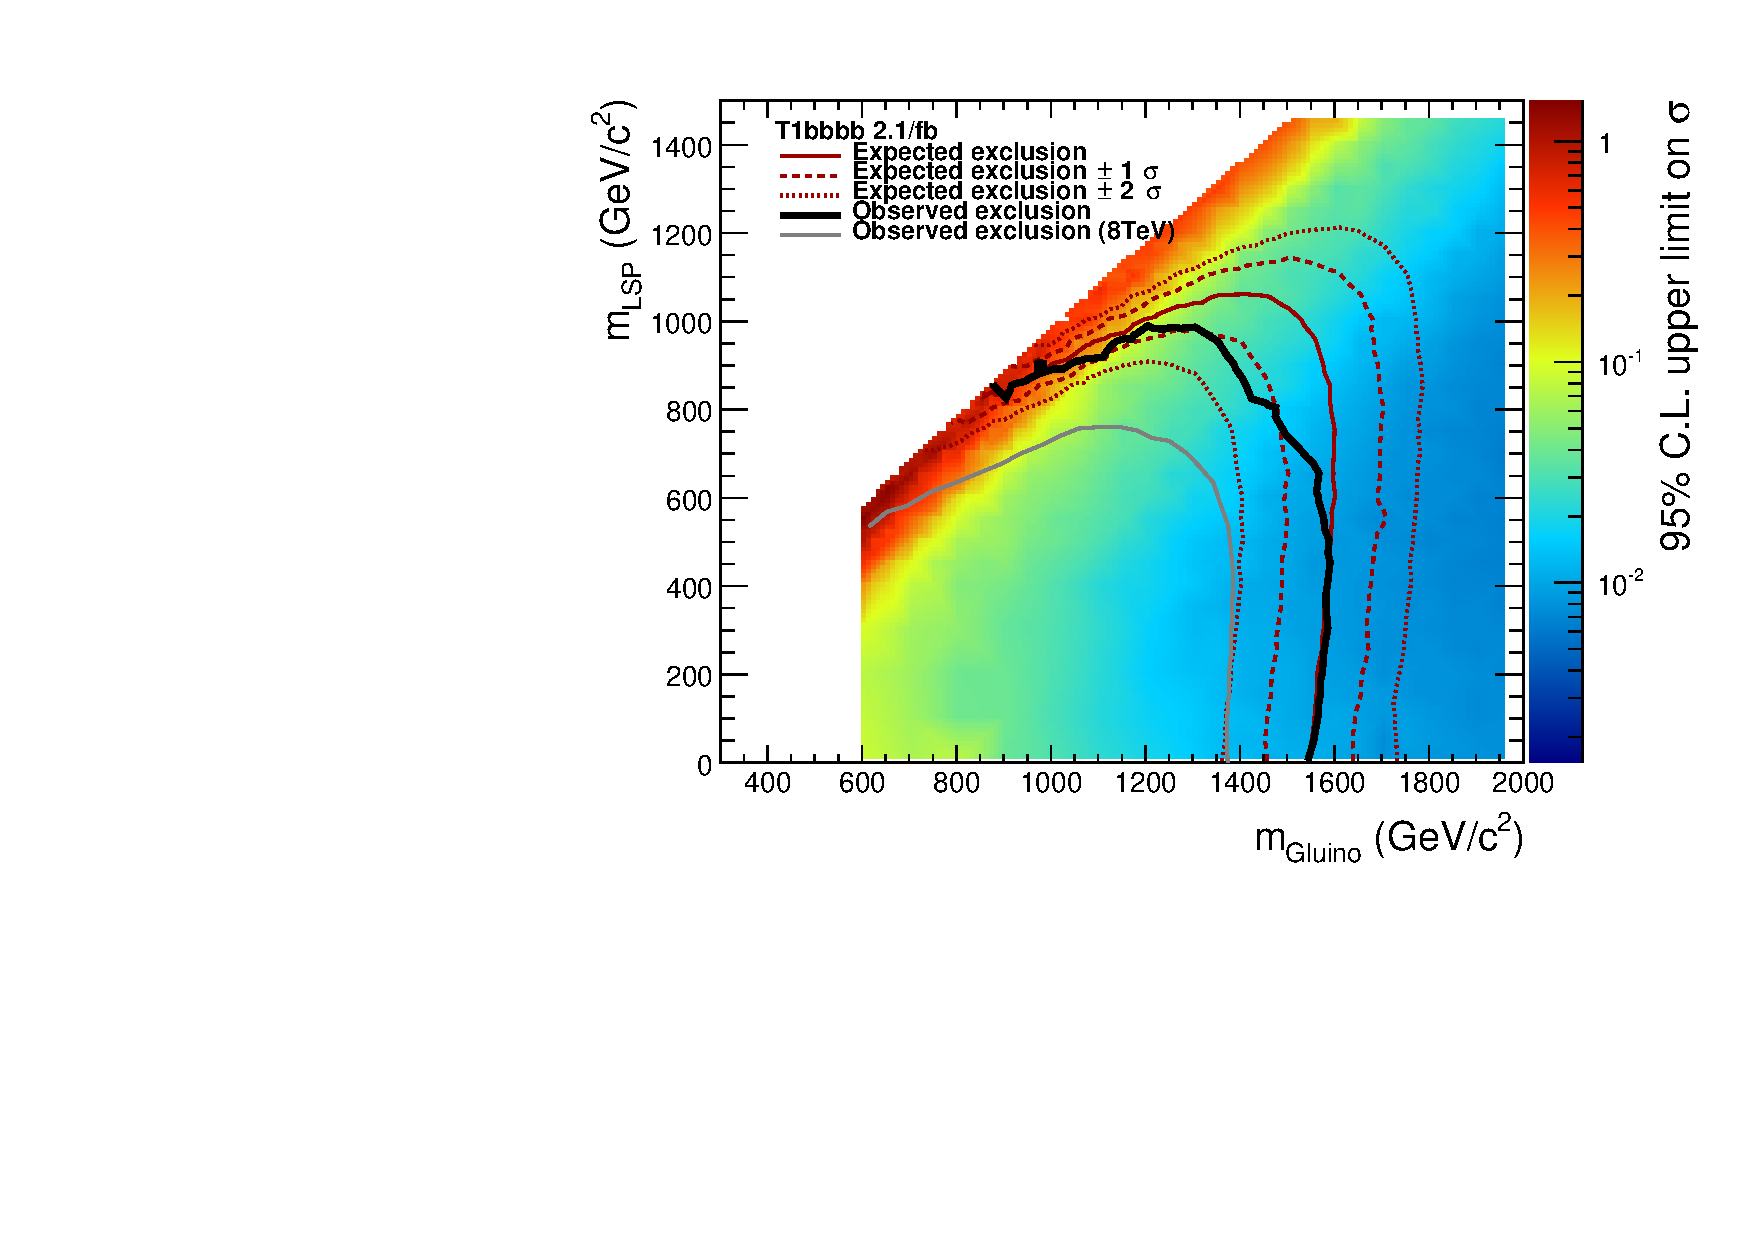
\includegraphics[width=0.8\textwidth]{xs_contour_withHisto.pdf}
    \caption{Observed upper limit on the gluino pair-production cross section at 95\% CL (indicated by the colour scale) as a function of the gluino
      and $\chiz$ masses for gluino three body decays to $bb\chiz$
      The red solid thick line represents the observed exclusions when
      varying the production cross section by its theoretical uncertainty. 
      The black solid line (thin dashed) line indicates the median (${\pm}1 \sigma$ 
      experimental uncertainty) expected exclusion.
      \label{fig:limits-sms} }
  \end{center}
\end{figure*}


Figure~\ref{fig:limits-sms} shows the observed upper limit on the
production cross section at 95\% confidence level (CL) as a function
of the gluino and LSP masses for
a range of simplified models assuming pair production of gluinos. The analysis places stringent limits in the mass parameter space, for example in the decay to $b$-quarks, gluino masses below 1.8~\TeV are excluded for LSP masses below about 800~\gev.
The observed excluded regions are determined with NLO+NLL
cross sections for gluino pair production assuming decoupled squarks. Also shown are the
observed excluded regions when varying the production cross section by
its theoretical uncertainty, and the expected excluded region with
both the ${\pm}1$ and ${\pm}2$ standard-deviation ($\sigma$)
variations. 

%%__________________________________________________________________||
